%%%%%%%%%%%%%%%%%%%%%%%%%%%%%%%%%%%%%%%%%%%%%%%%%%%%%%%%%%%%%%%%%%%%%%%%%%%%%%%%
%%%%%%%%%%%%%%%%%%   Vorlage für eine Abschlussarbeit   %%%%%%%%%%%%%%%%%%%%%%%%
%%%%%%%%%%%%%%%%%%%%%%%%%%%%%%%%%%%%%%%%%%%%%%%%%%%%%%%%%%%%%%%%%%%%%%%%%%%%%%%%

% Erstellt von Maximilian Nöthe, <maximilian.noethe@tu-dortmund.de>
% ausgelegt für lualatex und Biblatex mit biber

% Kompilieren mit
% latexmk --lualatex --output-directory=build thesis.tex
% oder einfach mit:
% make

%Das war meine BA
%\documentclass[
%%  tucolor,       % remove for less green,
%  BCOR=12mm,     % 12mm binding corrections, adjust to fit your binding
%  parskip=half,  % new paragraphs start with half line vertical space
%  open=any,      % chapters start on both odd and even pages
%  cleardoublepage=plain,  % no header/footer on blank pages
%]{tudothesis}

%Das ist ein einfacheres Dokument
\documentclass[
  bibliography=totoc,     % Literatur im Inhaltsverzeichnis
  captions=tableheading,  % Tabellenüberschriften
  titlepage=firstiscover, % Titelseite ist Deckblatt
]{scrartcl}


% Warning, if another latex run is needed
\usepackage[aux]{rerunfilecheck}

% just list chapters and sections in the toc, not subsections or smaller
\setcounter{tocdepth}{2}

%------------------------------------------------------------------------------
%------------------------------ Fonts, Unicode, Language ----------------------
%------------------------------------------------------------------------------
\usepackage{fontspec}
\defaultfontfeatures{Ligatures=TeX}  % -- becomes en-dash etc.

% german language
\usepackage{polyglossia}
\setdefaultlanguage{german}

% for english abstract and english titles in the toc
\setotherlanguages{english}

% intelligent quotation marks, language and nesting sensitive
\usepackage[autostyle]{csquotes}

% microtypographical features, makes the text look nicer on the small scale
\usepackage{microtype}

%------------------------------------------------------------------------------
%------------------------ Math Packages and settings --------------------------
%------------------------------------------------------------------------------

\usepackage{amsmath}
\usepackage{amssymb}
\usepackage{mathtools}

% Enable Unicode-Math and follow the ISO-Standards for typesetting math
\usepackage[
  math-style=ISO,
  bold-style=ISO,
  sans-style=italic,
  nabla=upright,
  partial=upright,
]{unicode-math}
\setmathfont{Latin Modern Math}

% nice, small fracs for the text with \sfrac{}{}
\usepackage{xfrac}


%------------------------------------------------------------------------------
%---------------------------- Numbers and Units -------------------------------
%------------------------------------------------------------------------------

\usepackage[
  locale=DE,
  separate-uncertainty=true,
  per-mode=symbol-or-fraction,
]{siunitx}
\sisetup{math-micro=\text{µ},text-micro=µ}
\DeclareSIUnit{\nothing}{\relax}

%------------------------------------------------------------------------------
%-------------------------------- tables  -------------------------------------
%------------------------------------------------------------------------------

\usepackage{booktabs}       % \toprule, \midrule, \bottomrule, etc
\usepackage{multirow}
\usepackage{tabularx}


%------------------------------------------------------------------------------
%-------------------------------- graphics -------------------------------------
%------------------------------------------------------------------------------

\usepackage{graphicx}
\usepackage{grffile}

% allow figures to be placed in the running text by default:
\usepackage{scrhack}
\usepackage{float}
\floatplacement{figure}{htbp}
\floatplacement{table}{htbp}

% keep figures and tables in the section
\usepackage[section, below]{placeins}


%------------------------------------------------------------------------------
%---------------------- customize list environments ---------------------------
%------------------------------------------------------------------------------

\usepackage{enumitem}

%------------------------------------------------------------------------------
%------------------------------ Bibliographie ---------------------------------
%------------------------------------------------------------------------------

\usepackage[
  backend=biber,   % use modern biber backend
  autolang=hyphen, % load hyphenation rules for if language of bibentry is not
                   % german, has to be loaded with \setotherlanguages
                   % in the references.bib use langid={en} for english sources
  sorting=none,
]{biblatex}
\addbibresource{lit.bib}  % the bib file to use
\DefineBibliographyStrings{german}{andothers = {{et\,al\adddot}}}  % replace u.a. with et al.

%------------------------------------------------------------------------------
%----------------------    das hab ich hinzugefügt   --------------------------
%------------------------------------------------------------------------------

\usepackage{geometry}
\usepackage{caption}
\usepackage{subcaption}
\usepackage[version=4]{mhchem}
\usepackage{tabularx}
\usepackage{multirow}
\usepackage{ulem}
\usepackage{color, colortbl}
\definecolor{Lightgray}{rgb}{0.8, 0.8, 0.8}
\definecolor{tu}{rgb}{0.196, 0.44, 0.00}

\addto\captionsngerman{%
  \renewcommand{\figurename}{Abb.}%
  \renewcommand{\tablename}{Tab.}%
}
\usepackage{lscape}
\newcommand*\cleartoleftpage{%
  \clearpage
  \ifodd\value{page}\hbox{}\newpage\fi
}

% Erweiterung zum Erstellen von Feynman-Diagrammen
\usepackage[compat=1.1.0]{tikz-feynman}

% Micro in \SI{}{} reparieren
\sisetup{math-micro=\text{µ},text-micro=µ}

% Code als Anhang
\usepackage{listings}
\lstset{
  backgroundcolor=\color{white},   % choose the background color; you must add \usepackage{color} or \usepackage{xcolor}; should come as last argument
  basicstyle=\footnotesize,        % the size of the fonts that are used for the code
  breakatwhitespace=false,         % sets if automatic breaks should only happen at whitespace
  breaklines=true,                 % sets automatic line breaking
  captionpos=b,                    % sets the caption-position to bottom
  commentstyle=\color{gray},    % comment style
  deletekeywords={...},            % if you want to delete keywords from the given language
  escapeinside={\%*}{*)},          % if you want to add LaTeX within your code
  %extendedchars=true,              % lets you use non-ASCII characters; for 8-bits encodings only, does not work with UTF-8
  firstnumber=0,                % start line enumeration with line 1000
  frame=single,	                   % adds a frame around the code
  keepspaces=true,                 % keeps spaces in text, useful for keeping indentation of code (possibly needs columns=flexible)
  keywordstyle=\color{blue},       % keyword style
  language=Python,                 % the language of the code
  morekeywords={*,...},            % if you want to add more keywords to the set
  numbers=left,                    % where to put the line-numbers; possible values are (none, left, right)
  numbersep=5pt,                   % how far the line-numbers are from the code
  numberstyle=\tiny\color{gray}, % the style that is used for the line-numbers
  rulecolor=\color{black},         % if not set, the frame-color may be changed on line-breaks within not-black text (e.g. comments (green here))
  showspaces=false,                % show spaces everywhere adding particular underscores; it overrides 'showstringspaces'
  showstringspaces=false,          % underline spaces within strings only
  showtabs=false,                  % show tabs within strings adding particular underscores
  stepnumber=2,                    % the step between two line-numbers. If it's 1, each line will be numbered
  stringstyle=\color{green},     % string literal style
  tabsize=2,	                   % sets default tabsize to 2 spaces
  title=\lstname                   % show the filename of files included with \lstinputlisting; also try caption instead of title
}

\author{%
  Katharina Brägelmann\\%
  \href{mailto:katharina.braegelmann@tu-dortmund.de}{katharina.braegelmann@tu-dortmund.de}%
  \texorpdfstring{\and}{,}%
  Lars Kolk\\%
  \href{mailto:lars.kolk@tu-dortmund.de}{lars.kolk@tu-dortmund.de}%
}
\publishers{TU Dortmund – Fakultät Physik}

%------------------------------------------------------------------------------
%------------------------------ Bibliographie ---------------------------------
%------------------------------------------------------------------------------

% Last packages, do not change order or insert new packages after these ones
%\usepackage[pdfusetitle, unicode, linkbordercolor=tugreen]{hyperref}
\usepackage[pdfusetitle, unicode]{hyperref}
\usepackage{bookmark}
\usepackage[shortcuts]{extdash}


%------------------------------------------------------------------------------
%-------------------------    Angaben zur Arbeit   ----------------------------
%------------------------------------------------------------------------------

%\author{Katharina Brägelmann}
%\title{Gasadsorption an geladenen Lipidmonolagen}
%\date{2019}
%\birthplace{Maastricht}
%\chair{Lehrstuhl für Experimentelle Physik I}
%\division{Fakultät Physik}
%\thesisclass{Bachelor of Science}
%\submissiondate{01. Juli 2019}
%\firstcorrector{Prof.~Dr.~Metin Tolan}
%\secondcorrector{Prof.~Dr.~Heinz Hövel}

\usepackage{longtable}
\usepackage{wrapfig}
\usepackage{ dsfont }
\subject{VERSUCH 18}
\title{Hochreine Germaniumdetektoren in der\\ \texorpdfstring{$\gamma$}. - Spektrometrie}
\date{%
  \hspace{-2.5em}
  Durchführung: 09.12.2019
  \hspace{4em}
  Abgabe: 06.01.2020
}

\begin{document}
  \setlength{\parindent}{0em}
  \maketitle
  \thispagestyle{empty}
  \newpage
  \tableofcontents
  \newpage
\section{Zielsetzung}
In diesem Versuch sollen mithilfe der Röntgenreflektometrie die Dichte, Rauigkeit und Schichtdicke eines dünnen Polystyrolfilms untersucht werden.
\subsection{Einleitung}
Der Zeeman-Effekt beschreibt die Aufspaltung und Polarisation von Spektrallinien eines Atoms unter Einfluss eines äußeren Magnetfeldes.
Durch das Aufspalten der diskreten Energieniveaus kommt es bei der Lichtemission zu kleinen Unterschieden in der Wellenlänge.

\subparagraph{Magnetisches Moment}
Hüllenelektronen können mit dem Bahndrehimpuls $\vec{l}$ und mit dem Eigendrehimpuls $\vec{s}$ beschrieben werden.
Dabei gilt:
\begin{align*}
  |\vec{l}|=\sqrt{l(l+1)}\hbar&& \text{mit } l &= 0,1,2,...,n-1\\
  |\vec{s}|=\sqrt{s(s+1)}\hbar&& \text{mit } s &= \frac{1}{2}.
\end{align*}
Die magnetischen Momente, welche durch die Drehimpulse und die Ladung der Elektronen entstehen, können beschrieben werden mit:
\begin{align*}
  \vec{\mu}_l &= -\mu_B \frac{\vec{l}}{\hbar} = -\mu_B \sqrt{l(l+1)}\vec{l}_e\\
  \vec{\mu}_s &= -g_S \frac{\mu_B}{\hbar}\vec{s} = -g_S \mu_B \sqrt{s(s+1)}\vec{s}_e.\\
\end{align*}
$\vec{l}_e$ und $\vec{s}_e$ sind die Einheitsvektoren in die jeweilige Richung.
Die Größe $g_S$ ist der Landé-Faktor. $\mu_B$ beschreibt das Bohrsche Magneton und ist dabei gegeben als:
\begin{align*}
  -\frac{1}{2} e_0 \frac{\hbar}{m_0}.
\end{align*}
Weiter gilt, dass $e_0$ die Elementarladung und $m_0$ die Elektronenmasse beschreibt.

\subsection{Wechselwirkung der Drehimpulse und magnetischer Momente untereinander}
Für Atome mit mehreren Elektronen gibt es viele unterschiedliche Arten, wie Bahndrehimpuls und Spin miteinander wechselwirken können.
Im Wesentlichen sind können zwei einfache Grenzfälle betrachtet werden, welche häufig in der Natur vorkommen.
%
Für Atome mit niedriger Kernladungszahl kann der Gesammtdrehimpuls $\vec{L}$ der Hülle aus den Bahndrehimpulsen $\vec{l}$ vektoriell zusammengesetzt werden.
Das liegt an der großen Wechselwirkung zwischen den Bahndrehimpulsen.
\begin{align*}
  \vec{L} = \sum_i{\vec{l}_i} \text{ mit } |\vec{L}|= \sqrt{L(L+1)}\hbar
\end{align*}
Für den Gesamtbahndrehimpuls müssen nur unabgeschlossene Schalen betrachtet werden, da abgschlossene Schalen immer einen Bahndrehimpuls von 0 besitzen.
$\vec{l}$ kann dabei nur ganzzahlige Quantenzahlen von 0,1,2 oder 3 annehmen.
Je nach Quantenzahl kann zwischen S,P,D und F-Term unterschieden werden.
Das magnetische Moment $\vec{\mu}_L$ vom Gesamtbahndrehimpuls $\vec{L}$ lässt sich errechnen mit:
\begin{align*}
  |\vec{\mu}_L| = \mu_B\sqrt{L(L+1)}.
\end{align*}
%
Für den Gesamtspin der Elektronenhülle $\vec{S}$ gilt für Atome mit niedriger Ordnungszahl ebenfalls die vektorielle Summation der einzelnen Komponenten.
Die Einzelkomponenten sind hier die Einzelspins $\vec{s}_i$.
\begin{align*}
  \vec{S} = \sum_{i}{\vec{s}_i}
\end{align*}
Die Gesamtspinquantenzahl $S$ kann der Werte $\frac{N}{2}, \frac{N}{2}-1, ..., \frac{1}{2},0$ annehmen.
$N$ beschreibt dabei die Anzahl der Elektronen aus den unabgeschlossenen Schalen.
Der Betrag des Gesamtspins lässt sich aufstellen zu:
\begin{align*}
  |\vec{S}| = \sqrt{S(S+1)}\hbar.
\end{align*}
Der dazugehörige Betrag des magnetischen Momentes ist gegeben als:
\begin{align*}
  |\vec{\mu}_S| = g_S\mu_B\sqrt{S(S+1)}.
\end{align*}
Im Falle, dass das Atom keinem zu großen Magnetfeld ausgesetzt ist kann der Gesammtdrehimpuls $\vec{J}$ geschrieben werden als:
\begin{align*}
  \vec{J} = \vec{L}+ \vec{S}.
\end{align*}
Die beschriebene LS-Kopplung ist für die Betrachtung des Zeeman-Effekts zugrunde gelegt.
$\vec{J}$ kann abhängig von $S$ ganz- oder habzahlig sein.
Der Betrag vom Gesamtdrehimpuls ist gegeben als:
\begin{align*}
  |\vec{J}| = \sqrt{J(J+1)}\hbar.
\end{align*}
Beschreibt man ein Energienivau, kann das mit der Darstellung
\begin{align*}
  {}^M\mathcal{L}_J
\end{align*}
erfolgen.
$M$ ist dabei die Multiplizität und von $S$ abhängig in der Form $M=2S+1$.
Für das Drehimpulssymbol $\mathcal{L}$ gilt:
$\mathcal{L}\in\{S(L=0), P(L=1), D(L=2), F(L=3)\}$.
Wobei $L$ wieder der Gesamtdrehimpuls ist.\\
%
Der zweite Grenzfall betrachtet die j-j-Kopplung bei Atomen mit höheren Kernladungszahlen.
Durch die starke Kopplung zwischen den Spin und den Bahndrehimpuls eines Einzelelektrons setzt sich der Gesamtdrehimpuls des Elektrons nun zusammen aus:
\begin{align*}
  \vec{j}_i = \vec{l}_i + \vec{s}_i.
\end{align*}
Der gesammt Drehimpuls der Elektronenhülle lässt sich schreiben als:
\begin{align*}
  \vec{J}=\sum_i\vec{j}_i.
\end{align*}
Es bei dieser Betrachtung kann kein Gesammtdrehimpuls $\vec{L}$ oder ein Gesamtspin $\vec{S}$ definiert werden.\\
Für Atome mit mittlerer Kernadungszahl besteht ein fließender Übergang zwischen den beiden Grenzfällen.
\FloatBarrier

\subsection{Aufspaltung der Energienivaus eines Atoms im homogenen Magnetfeld}
%
\begin{figure}[h!]
  \centering
  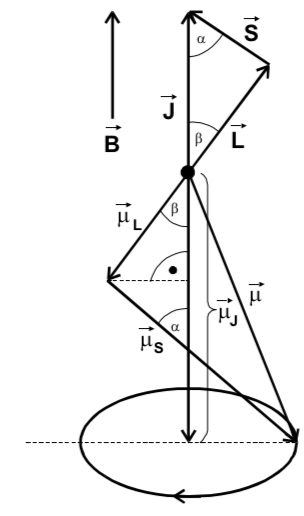
\includegraphics[width=5cm]{magmom1.png}
  \caption{Darstellung der verschiedenen magnetischen Momente von Spin, Bahndrehimpuls und Gesamtdrehimpuls}
  \label{fig:mag}
\end{figure}
%
Das magnetische Moment, welches zum Gesammtdrehimpuls $\vec{J}$ gehört, lässt sich berechnen mit
\begin{align*}
  \vec{\mu}_J&=\mu_Bg_J\sqrt{J(J+1)},
\end{align*}
wobei für den Landé-Faktor $g_J$ des entsprechenden Atoms gilt:
\begin{align}
		g_J:=&\frac{3J(J+1)+S(S+1)-L(L+1)}{2J(J+1)}.
\end{align}
\FloatBarrier

\subsection{Energieaufspaltung und Übergänge}
Durch die Richtungsquantelung sind nur genau $2J+1$ Einstellungen des atomaren magnetischen Momentes zu der äußeren Feldrichtung möglich.
Die zusätzliche Energie, die das Moment $\vec{\mu}$ im äußeren Magntfeld bekommt, ist gegeben als:
\begin{align*}
  E_{\text{mag}} = -\vec{\mu}_J \cdot \vec{B} = mg_J\mu_B.
\end{align*}
Für die Orientierungsquantenzahl $m$ gilt $-J < m < J$.
Für den Fall, dass $B \ne 0$ spaltet sich also das Enaginiveau $E_0$ eines Atoms auf in $2J+1$ äquidistante Niveaus.
%In der Abbildung %\ref{fig.J2}
%ist diese Aufspaltung für $J = 2$ abgebildet.
%\begin{figure}[h!]
%	\centering
%	\includegraphics[width=0.6\textwidth]{Aufspaltung.pdf}
%	\caption{Aufspaltung eines Energieniveaus von einem Atom mit $J=2$. \cite{V27}}\label{fig:J2}
%\end{figure}
Die Aufspaltung führt bei Lichtemission zur Aufspaltung des Spektrums, diese wird als Zeeman-Effekt bezeichnet.
%
Da nur bestimmte Energieübergänge möglich sind, gibt es die Auswahlregeln.
%
Für die Festlegung der Auswahlregeln wird die zeitabhängige Schrödingergleichung benötigt.
\begin{align}
	-\frac{\hbar^2}{2m}\Delta \psi(\vec{r},t)+U\psi(\vec{r},t)-i\hbar\frac{\partial \psi(\vec{r},t)}{\partial t}=0.
\end{align}
Die Lösungen $\psi$ beschreiben den Übergang zwischen den Energieniveaus $\alpha$ und $\beta$.
Aus den Lösungen ergibt sich eine Schwingung des Elektrons zwischen den beiden Energieniveaus mit der Frequenz:
\begin{align*}
  \nu_{\alpha\beta}:=\frac{E_\alpha-E_\beta}{h}.
\end{align*}
Das Elektron lässt sich dementsprechend als Dipol beschreiben, welches in die $x$-Richtung mit:
\begin{align*}
  	D_x=-e_0\text{const } 2 \Re \real\left( \underbrace{\int x\psi^*_\beta\psi_\alpha dV}_{x_{\alpha\beta}}\exp(2\pi i\nu_{\alpha,\beta}t) \right)
\end{align*}
abstrahlt.
Für die $y$ und $z$ Richtung kann die Formel analog aufgestellt werden.
Das Integal $x_{\alpha\beta}$ und seine analogen $y$ und $z$ Komponenten werden Matxixelemente bezeichnet und sind wichtig für die berechnung des Poynting-Vektors $\vec{S}_{\alpha\beta}$.
Der Poyning-Vektor berechnet sich nach:
\begin{align*}
  |\vec{S}_{\alpha\beta}| \sim \left(|x_{\alpha\beta}|^2+|y_{\alpha\beta}|^2+|z_{\alpha\beta}|^2\right) \text{sin}^2(\gamma).
\end{align*}
$\gamma$ beschreibt dabei den Winkel zwischen Dipolmoment und Ausbreitungsrichtung der Strahlung.
Es kann gezeigt werden, dass die Intensität der vom Dipol emittierten Strahlung mit den Matixelementen zusammenhängt.
Für den Fall, dass das B-Feld in die Z-Richtung zeigt, verschwindet $z_{\alpha\beta}$, außer wenn gilt, dass $m_{\alpha} = m_{\beta}$.
$x_{\alpha\beta}\pm i y_{\alpha\beta}$ verschwindet ebenfalls, außer wenn gilt, dass $m{\beta} = m_{\alpha} \pm 1$.
Zum Zeeman-Effekt kommt es also nur, wenn sich die Orientierungsquantenzahlen $m_{\alpha}$ und $m_{\beta}$ gar nicht oder nur um $\pm 1$ unterscheiden.\\
%
Für den Fall, dass $\Delta m = 0$ ($z_{\alpha\beta} \neq 0,\ x_{\alpha\beta} = i y_{\alpha\beta} = 0$) kommt es Schwingung des Dipols parallel zu Magnetfeldachse,
dies führt bei der Emission zu linear-polarisiertem Licht parallel zu $\vec{B}$.
Durch die Polarisation kann das emittierte Licht am besten senkrecht (Transversal) zur Feldrichtung beobachtet werden.
Die Strahlungsart wird als $\pi$ bezeichnet.\\
%
Für den Fall, das $\Delta m = \pm 1$ ($z_{\alpha\beta} = 0,\ x_{\alpha\beta} = \pm i y_{\alpha\beta} \neq 0$) kommt es zu links oder rechts zirkular-polarisierter Stahlung um die Magnetfeldachse.
Bei Betrachtung aus der transversalen Achse zur Feldachse erscheint emittiertes Licht linear polarisiert.
Die Strahlungsarten werden als $\sigma$ bezeichnet.
%
Die oben getroffenen Aussagen gelten nur für den Fall, dass $S=0$.
Diesen Spezialfall bezeichnet man als normalen Zeeman-Effekt.
Für Übergänge mit $S=0$ gilt $g_J = 1$. Die Verschiebung der Energieniveaus ist dementsprechend unabhängig von den Quantenzahlen.
Der Energieunterschied $\Delta E$ zwischen den Niveaus ist unabhängig von $L$ und $J$ gleich groß.
\begin{align}
  \Delta E = m \mu_B B \text{ für } -J \leq m \leq J
  \label{eqn:normal}
\end{align}

Der anormale Zeeman-Effekt kommt deutlich häufiger vor und tritt auf, wenn $S \neq 0$.
Es gelten für die Übergänge die selben Auswahlregeln $\Delta m = 0, \pm 1$.
Da $g_J = 1$ nicht mehr gegeben ist, ergeben sich für die Übergänge die Energien von:
\begin{align}
	E=(m_ig_{J_i}-m_jg_{J_j})\mu_BB+E_0.
  \label{eqn:anormal}
\end{align}
\FloatBarrier

\subsection{Vorbereitungsaufgabe}
\begin{figure}[h!]
  \centering
  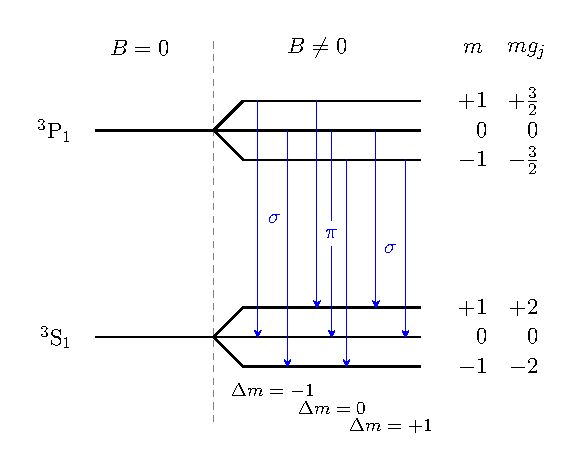
\includegraphics[width=9cm]{termschema_blau.pdf}
  \caption{Termschema eines ${}^3P_1\leftrightarrow {}^3S_1$ Übergangs. Der Übergang liegt im blauen Wellenlängenbereich.}
  \label{fig:blau}
\end{figure}
\begin{figure}[h!]
  \centering
  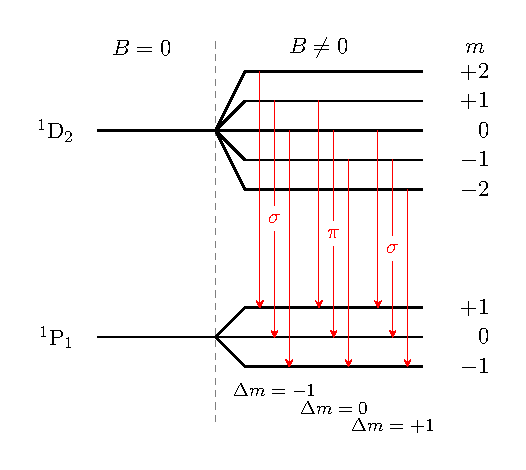
\includegraphics[width=9cm]{termschema_rot.pdf}
  \caption{Termschema eines ${}^1D_2 \leftrightarrow {}^1P_1$ Übergangs. Der Übergang liegt im roten Wellenlängenbereich.}
  \label{fig:rot}
\end{figure}
\FloatBarrier
\begin{table}
	\centering
	\begin{tabular}{cccccc}
		\toprule
		Übergang & $m_1$  & $g_{1}$ & $m_2$ & $ g_2$ & $g_{12}$\\
		\midrule
		& \multicolumn{2}{c}{${}^1P_1$}  & \multicolumn{2}{c}{${}^1D_2$} \\
		\midrule
		& 2 & 1 & 1 & 1 & 1\\
		$\sigma$& 1 & 1 & 0 & 1 & 1\\
		& 0 & 1 & -1 & 1 & 1\\
		\midrule
		& 1 & 1 & 1 & 1 & 0\\
		$\pi$ & 0 & 1 & 0 & 1 & 0\\
		& -1 & 1 & -1 & 1 & 0\\
		\midrule
		& 0 & 1 & 1 & 1 & -1\\
		$\sigma$ & -1 & 1 & 0 & 1 & -1\\
		& -2 & 1 & -1 & 1 & -1\\\bottomrule
	\end{tabular}
	\caption{Hier sind die Landé-Faktoren der roten Spektrallinie aufgeführt.}
	\label{tab:Lande_rot}
\end{table}
\begin{table}
	\centering
	\begin{tabular}{cccccc}
		\toprule
		Übergang & $m_1$  & $g_{1}$ & $m_2$ & $ g_2$ & $g_{12}$\\
		\midrule
		& \multicolumn{2}{c}{${}^3S_1$}  & \multicolumn{2}{c}{${}^3P_2$} \\
		\midrule
		$\sigma$ & +1 & 2 & 0 & $\frac{3}{2}$& 2\\
		& 0 & 2 & -1 & $\frac{3}{2}$ & $\frac{3}{2}$\\
		\midrule
		& +1 & 2 & +1 & $\frac{3}{2}$ & $\frac{1}{2}$\\
		$\pi$ & 2 & 2 & 0 & $\frac{3}{2}$ & 0 \\
		& -1 & 2 & -1 & $\frac{3}{2}$ & -$\frac{1}{2}$\\
		\midrule
		& 0 & 2 & 1 & $\frac{3}{2}$ & -$\frac{3}{2}$\\
		$\sigma$ & -1 & 2 & 0 & $\frac{3}{2}$& -2\\
		\bottomrule
	\end{tabular}
	\caption{Hier sind die Landé-Faktoren der blauen Spektrallinie aufgeführt.}
	\label{tab:Lande_blau}
\end{table}
\FloatBarrier

\section{Aufbau}
Der Aufbau des zylinderförmigen Germaniumdetektors ist in Abbildung \ref{fig:Aufbau} dargstellt. Wie dort zu sehen ist, besteht die Oberfläche des Detektors aus einer mit Lithium dotierten $n$-Schicht die als $+$-Pol dient. Im inneren des Detektorkristalls befindet sich eine koaxiliale Bohrung. Deren innere Oberfläche wurde mit Gold bedampft und stellt somit eine $p$-dortierte Schicht da. Zwischen diesen Schichten befindet sich ein reiner Germaniumkristall, in dem sich aufgrund der $p$ - und $n$-dotierten Schichten zur Ausbildung einer ausgedehnten Verarmungszone kommt. 
\begin{figure}[H]
    \centering
    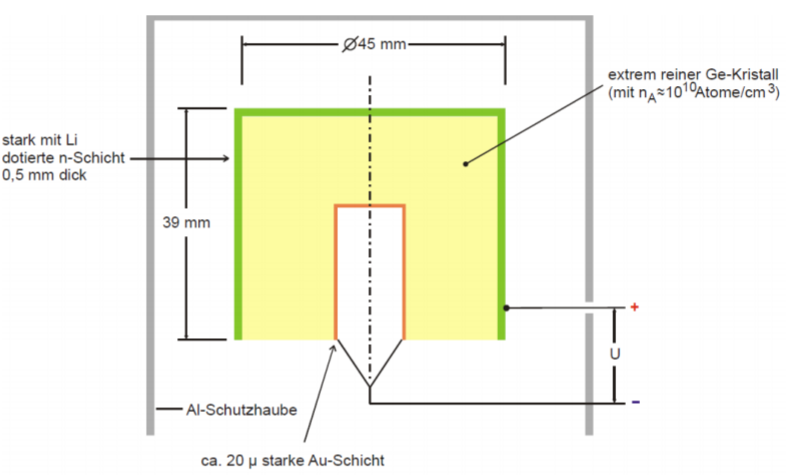
\includegraphics[width=0.8\textwidth]{content/images/Aufbau.png}
    \caption{Koaxialquerschnitt des Detektors \cite{anleitung} }
    \label{fig:Aufbau}
\end{figure}
Einfallende Photonen müssen zuerst die Aluminium-Schutzhaube durchqueren, die den Detektor umgibt, bevor an die $n$-dotierte Schichte gelangen. Daher existiert eine untere Nachweisgrenze von $40-50 \si{\kilo \electronvolt}$ sowie eine Vollenergienachweisgrenze von ca. $150 \si{\kilo \electronvolt}$ für Photonen.

\section{Durchführung}
Zunächst wird ein $^{152}\symup{Eu}$-Strahler mit bekannter Aktivität dazu verwendet, den Detektor zu kalibrieren und die Vollenergienachweiswahrscheinlichkeit zu bestimmen. Anschließend werden die Aktivitäten von $^{137}\symup{Cs}$- und  $ ^{133}\symup{Ba} $ Proben mit dem Detektor untersucht. Zum Schluss wird die Aktivität einer unbekannten Probe untersucht, um auf die Probe zurückzuschließen. 
\section{Auswertung}
\begin{itemize}
	\item Gauss an Detektorfunktion -> FWHM, max. Intensität
	\begin{equation*}
		\frac{a}{\sqrt{2 \pi \sigma^2}} \, \exp{\left(-\frac{\left(x-\mu \right)^2}{2 \sigma^2}\right)}+c
	\end{equation*}
	\begin{align}
		Amp && \mu && \sigma && c \\
		1.02109927e+05 && 4.73463215e-04 && 4.34837954e-02 && 1.35592289e+04 \\
		1.08925087e+03 && 4.71014525e-04 && 4.93489841e-04 && 2.24293788e+03 \\
	\end{align}
	\item messung - diffus abgebildet\\
	Geometriewinkel \colorbox{green}{$\alpha = \arcsin{\left( \frac{d}{D}\right)} = \SI{0.5729673448571527}{°}$} mit $d=\SI{0.2}{mm}$ und $D=\SI{0.02}{m}$\\
	Für kleinere Winkel als den Geometriewinkel ($\alpha_i < \alpha_G$) gilt $G = \frac{\sin{(\alpha_i)}}{\sin{(\alpha_G)}}$ für größere Winkel gilt $G=1$\\
	Geometriewinkel in die Daten eingebezogen, abgebildet
	\item $q_z=\frac{4\pi}{\lambda}\sin{(\alpha_i)}$, $\lambda = \SI{1.54e-10}{m}$
	\item Wie zeichne ich die idealglatte OF?
	\item Strahlbreite und Probenlänge aus Geometriewinkel berechnen -> wie kriege ich den Geometriewinkel aus den Daten?\\
	haha, im ersten Rockingscan sind die Daten ab $\SI{-0.44}{°}$ bzw. $\SI{0.56}{°}$ relevant unterscheidbar von 0\\
	Mittelwert des Betrags: \colorbox{yellow}{$\SI{0.5}{°}$} \\
	Vgl (rel. Abw. (grün-gelb)/gelb): $\SI{14.59}{\%}$
\end{itemize}

Im Versuch werden die Übergänge des Cadmiums unter Aufspaltung durch den Zeeman-Effekt betrachtet.
Dem roten Licht liegt dabei der normale Zeeman-Effekt zugrunde, dem blauen Licht der anormale Zeeman-Effekt.\\
Der Landé-Faktor des Übergangs $g_{12}$ ergibt sich für den normalen Zeeman-Effekt (rot) zu
\begin{equation*}
  g_{ij}  &= \SI{0.974 \pm 0.011}{}.
\end{equation*}
was mit einer relativen Abweichung von $f=\SI{2.65}{\%}$ zum theoretischen Landé-Faktor
\begin{equation*}
  g_{12, \text{theo}} = \SI{1}{}
\end{equation*}
des zirkularen Übergangs passt.
\begin{figure}[h!]
  \centering
  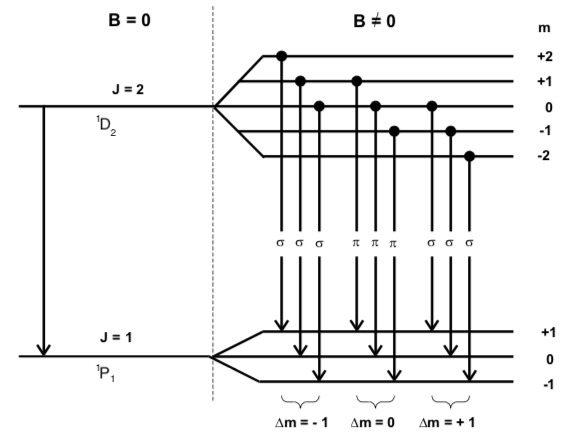
\includegraphics[width=\textwidth]{normal.png}
  \caption{Aufspaltung durch den normalen Zeeman-Effekt \cite{1}}
  \label{fig:normal}
\end{figure}
\FloatBarrier
Für die Übergänge des anormalen Zeeman-Effekts werden die Landé-Faktoren des Übergangs $g_{ij}=m_{1}g_{1}-m_{2}g_{2}$ berechnet und mit der Theorie verglichen.
Der theoretische Wert für $\sigma$ mittelt sich hier aus den Werten $g_{12, \text{theo}, 1}=2$ und $g_{12, \text{theo}, 2}=\frac{3}{2}$, da sich die Linien durch den optischen Doppler-Effekt stark überlagern, die Messung aber über die Mitte der Linie ausgeführt wird.
Wiederum der zweite theoretische Wert für den $\pi$-Übergang $g_{12, \text{theo}} = 0 $ ist stark unterdrückt und fällt im Mittel nicht ins Gewicht.
So ergibt sich:
\begin{align*}
  \sigma  &&& g_{12, \text{exp}} &= \SI{1.30 \pm 0.02}{}    &&&   g_{12, \text{theo}} &= \SI{1.75}{}     &&&  f=\SI{25.71}{\%}   \\
  \pi     &&& g_{12, \text{exp}} &= \SI{0.442 \pm 0.004}{}  &&&   g_{12, \text{theo}} &= \SI{0.5}{}   &&&  f=\SI{11.60}{\%}   .
\end{align*}
\begin{figure}[h!]
  \centering
  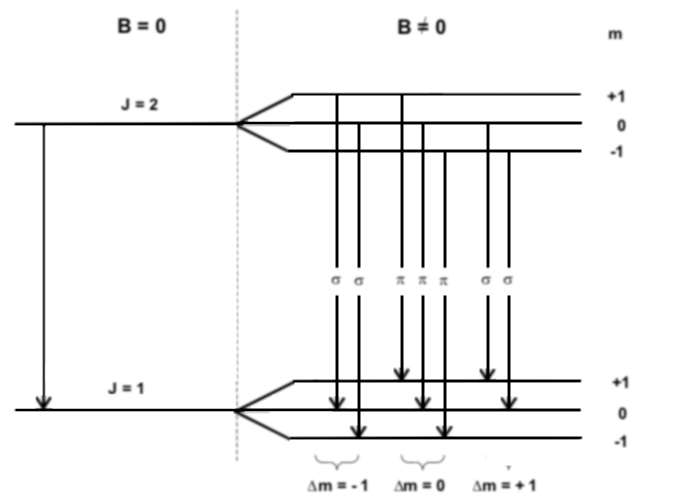
\includegraphics[width=\textwidth]{anormal.png}
  \caption{Aufspaltung durch den anormalen Zeeman-Effekt \cite{1}}
  \label{fig:normal}
\end{figure}
\FloatBarrier
Mögliche Erklärungen für die Abweichungen sind der bereits genannte optische Doppler-Effekt, 

\printbibliography{}
%\includepdf[pages=-]{Text/Bilder/Werte.pdf}

\end{document}
